\chapter{Methodology}
\label{chap:method}

In this section, the methodology of the proposed solution is explained in detail. This section is divided into sequential subsections that each describe a step in the process used to arrive at the proposed dataset, the formulation of the analytical problem to be solved, and the \acrfull{ml} related data preparation, training, and evaluation.

\section{General approach overview}

Based on the findings from the literature review conducted in \cref{sec:lit_review}, it is clear that the existing work is limited in terms of a general and global prediction solution for vessel destination ports. Thus, this thesis proposes a method that is able to predict vessels' future destination ports using a combination of positional data from the \gls{aivdm} protocol and vessel segmentation values. This is an important objective of the thesis as no related studies seem to take additional vessel information into account. The proposed solution is not restricted by specific geographical regions nor time intervals and should form a foundation of which it is possible to extend with more features, or data attributes, regarding the traveling vessels and voyages. The method of developing the proposed solution can be divided into the following steps:

\begin{enumerate}
    \item Construct voyages and trajectories using a voyage definition derived from the departure and arrival detection described in \cref{sec:vessel_transitions}.
    \item Sample, or simplify, the trajectories to make them more comparable using vessel similarity measurement methods.
    \item Calculate the \acrfull{mstd} and the similarity value for every voyage's trajectory.
    \item Collect the historical data attributes to be used for \acrfull{ml} including departure and arrival ports, vessel segmentation values, \acrshort{mstd} values, and trajectory lengths.
    \item Train a \acrshort{ml} model to predict the arrival ports of voyages using the dataset constructed.
\end{enumerate}

\section{The initial data processing}

This section describes the initial dataset used in the proposed solution which is later processed and used to train a \acrshort{ml} model for predictions. This data foundation is provided to the author by \acrfull{mo}. Moreover, for this thesis, data used in the analysis is stored in a separate, dedicated PostgreSQL database also hosted in \acrshort{mo}'s cloud computing environment.

\subsection{Positional historical AIS data}

The first step in the dataset processing is to collect a historical set of \acrshort{ais} data. In this thesis, this data provided by \acrshort{mo} contains more than 1.5 billion positional records for over 65 000 unique vessels starting from December 2019 and is continuously collected. In this thesis, circa 1.2 billion records ranging from December 2019 to March 2021 was used for the proposed solution. The historical records were copied in batches from \acrshort{mo}'s database into a separate database used in this thesis in a table called \textit{vessel positions history}. This table contains the following relevant attributes for each historical record:

\begin{itemize}
    \item id - a sequential identifier
    \item imo - the \acrshort{imo} number of the vessel that transmitted the position.
    \item mmsi - the \acrshort{mmsi} number of the vessel that transmitted the position.
    \item position - a geographical coordinate of the vessel in the \textit{Mercator} projection.
    \item timestamp - the UNIX timestamp (seconds since Unix Epoch) of when the position was transmitted by the vessel.
\end{itemize}

In the process of copying data to the dedicated database, each position's coordinate is validated by ensuring that it follows the bounds its projection, i.e., that the longitude value is between -180, and 180 degrees and the latitude is between -90, and 90 degrees. If a coordinate has invalid values, it is disregarded. Furthermore, positions that lie exactly on the north and south bounds, or exactly at coordinates \textit{(180, 90)} and \textit{(-180, -90)} are also disregarded as these positions are impossible places to navigate but are still frequently seen in the database. \cref{fig:ais_positions} in \cref{sec:ais_data} shows a visualization of an extract of 100 million records from the historical \acrshort{ais} database which shows the extent of the collected positions.

Furthermore, as also mentioned in \cref{sec:ais_data}, \acrshort{imo} numbers and \acrshort{mmsi} numbers are divided up in the positional and static \acrshort{ais} reports. Therefore, \acrshort{mmsi} numbers in positional data must be matched to \acrshort{imo} numbers in the static information (which contains both) to collect both identifiers in the historical \acrshort{ais} database. The \acrshort{imo} identifier is required to extract information such as vessel segments and sub-segments as these are initially constructed using information from static records. Positions transmitted by a \acrshort{mmsi} number that does not map to a known \acrshort{imo} number, or have invalid values for either, are disregarded. The validity of both values can be determined following the \gls{aivdm} protocol which defines how these numbers are constructed and used.

\subsection{Segments}

As described in \cref{sec:vessel_info_segments}, vessel segmentation values are additional attributes that indicate a vessel's type, dimensions, and capacity. These labels are thought to provide insight into the traveling patterns of vessels. Thus, this information is important for this thesis's proposed solution. \acrshort{mo} has vessel segmentation information for every unique vessel collected by \acrshort{ais} data. This information is collected and stored in the dedicated database in a table called \textit{vessel segments}. This table contains information per vessel and has the following relevant attributes:

\begin{itemize}
    \item imo - the \acrshort{imo} number of the vessel.
    \item segment - the vessel's segment value, e.g. \textit{dry bulk}, \textit{tanker}, \textit{chemical}, etc\ldots
    \item sub-segment - the vessel's sub-segment value, e.g., \textit{mini bulker}, \textit{handysize}, \textit{panamax}, etc\ldots
\end{itemize}

Finally, it is worth noting that some vessels can function as two different types of vessels such as tanker vessels that also function as chemical transport vessels. These ``combo'' vessels contain multiple entries in the segmentation database table for each of the functions it serves. However, they also contain a dedicated entry where the segment value is ``combo'' which can have a specific range of sub-segments. For analysis, it is more practical to assume that every vessel only has one segment and one sub-segment, therefore, for combo vessels, only the combo segment and sub-segment are considered.

\subsection{Ports}

Next, the traveling vessel's departure and arrival port are required to predict vessels' future destinations, as destinations are defined ports. As already described in \cref{sec:shipping_ports}, \acrshort{mo} has a large number of ports available in a port database out of which around 5600 are considered relevant for the shipping industry. For this thesis, only these 5600 relevant ports are considered for the analysis, thus, these are also stored in the dedicated database in a table called ``ports''. This table contains the following relevant attributes:

\begin{itemize}
    \item locode - the port's unique identifier following the \gls{locode} protocol.
    \item position - the port's geographical coordinates specified in the Mercator projection.
    \item name - a text value for the name of the port.
\end{itemize}

\subsection{Vessel transitions}

As described in \cref{sec:vessel_transitions}, vessel transitions are historical events where a vessel's \acrshort{ais} navigational status transitions from a status indicating that it is moving to the status ``MOORED'' and vice versa. These events are mapped geographically to the closest known port within a 25-kilometer radius, thus, vessel transitions provide a historical record of port arrivals and departures. \acrshort{mo} has more information available in their transition data, however, only vessel arrival and departure data are of relevance to the proposed solution. The relevant data is stored in the dedicated database as a table called \textit{vessel transitions}. This table contains vessel identifiers, the event's mapped port, the Unix timestamp of when the event occurred, and the transition type indicating whether the vessel arrived or departed. \cref{tab:vessel_transitions_example} shows an example extract from the transitions data for a single vessel. It shows that when sorted by time, the events follow a pattern of sequential arrival and departures from different ports.

\begin{table}[htbp]
    \centering
    \begin{tabular}{p{0.7in} p{0.9in} p{1in} p{1in} p{0.65in}}
    \hline
    \bfseries{IMO} & \bfseries{MMSI} & \bfseries{Transition} & \bfseries{Timestamp} & \bfseries{Port Code} \\ \hline
        9824083 & 538008866 & ARRIVAL   & 1595383670 & KRONS \\ \hline
        9824083 & 538008866 & DEPARTURE & 1596177702 & KRONS \\ \hline
        9824083 & 538008866 & ARRIVAL   & 1599869735 & BRITQ \\ \hline
        9824083 & 538008866 & DEPARTURE & 1600002777 & BRITQ \\ \hline
        9824083 & 538008866 & ARRIVAL   & 1603942962 & CNZNG \\ \hline
        9824083 & 538008866 & DEPARTURE & 1604191770 & CNZNG \\ \hline
    \end{tabular}
\caption{Example rows for a single vessel in the vessel transitions table}
\label{tab:vessel_transitions_example}
\end{table}

\section{Vessel voyage definition}

After the initial data foundation is constructed as described in the previous section, the next step is to construct voyages and voyage trajectories based on the historical \acrshort{ais} data. As described in \cref{sec:vessel_voyage_definition}, throughout this thesis, a vessel voyage has been defined based on vessel transitions derived from \acrshort{ais} navigational statuses. This is mainly because it is thought to provide more valuable predictions for the actors in the industry. This hypothesis was confirmed by the collaborative company \acrfull{mo}, but has also been corroborated by interviewing real actors in the industry as will be later discussed in \cref{chap:results}. This section describes the methods tested and used to construct voyages from the initial data foundation described up to this point in \cref{chap:method}.

\subsection{Cluster-based voyages}

\todo{Should I bother explaining work I did with clustering if I didn't use it in the final approach?}

\subsection{Transition voyages}

As vessel transitions provide a historical record per vessel of arrivals and departures based on \acrshort{ais} statuses it can be used to derive vessel voyages. Given two entries in the vessel transitions table for a single vessel, sorted by time, where the first is a departure from a port, and the second is arrival at another port, a voyage can be defined as starting at the timestamp of the first departure transition and ending at the subsequent arrival transition. For example, in \cref{tab:vessel_transitions_example}, there are six transition events for a single vessel ordered by time. Based on these events, two different voyages can be defined:

\begin{enumerate}
    \item  Vessel departed port \textit{KRONS} on the 31st of July 2020 and arrived at port \textit{BRITQ} on the 12th of September 2020.
    \item  Vessel departed port \textit{BRITQ} on the 13th of September 2020 and arrived at port \textit{CNZNG} on the 29th of October 2020.
\end{enumerate}

Using the vessel transition information, the first step is to deduce voyages based on sequential arrival and departures for vessels. After a voyage has been defined, the second step is to find the trajectory of the traveling vessel. This can be deduced from the vessel positions history table as every \acrshort{ais} positional report transmitted between the derived departure and arrival timestamps from the traveling vessel forms a geographical trajectory from the departure and arrival port.

\subsubsection{Constructing voyages}

Constructing voyages based on vessel transitions and positional records can be summarized in the following steps:

\begin{enumerate}
    \item Extract vessel transitions per vessel ordered by time.
    \item Define voyages based on subsequent departures and arrivals from the vessel transition data (\cref{lst:voyage_times}).
    \item For each voyage, extract every positional record between vessels' departure and arrival timestamps sorted by time.
    \item Validate the geographical trajectory including applying a ``noise filter'' (\cref{fig:noise_filter}).
    \item Store voyages with validated trajectories in transition voyages table.
\end{enumerate}

The first step including defining trajectories based on vessel transitions is a relatively straightforward process of looking for transitions following the pattern of departures immediately followed by arrival at a different port. The algorithm used to compute voyages based on a vessel's transition events is shown in \cref{lst:voyage_times}.

\begin{lstlisting}[
    caption={Golang code used to compute voyage times from vessel transitions. The code has been reduced slightly for readability.},
    label=lst:voyage_times,
    language=Go
]
func getVoyageTimes(transitions []VesselTransition) []Voyage {
	var voyages []Voyage
	j := 0
	for i, current := range transitions {
                // start at the first departure event
		if current.Transition != "DEPARTURE" {
			continue
                // get the subsequent transition
		j = i + 1
		if j >= len(transitions) {
			break
		}
		next := transitions[j]

                // ensure the next event is an arrival at a different port
		if next.Transition != "ARRIVAL" {
			continue
		}
		if current.PortCode == next.PortCode {
			continue
		}

		voyages = append(voyages, Voyage{
			IMO:                current.IMO,
			MMSI:               current.MMSI,
			DeparturePort:      current.PortCode,
			DepartureTimestamp: current.Timestamp,
			ArrivalPort:        next.PortCode,
			ArrivalTimestamp:   next.Timestamp,
		})
	}
	return voyages
}
\end{lstlisting}

Next, the voyage times computed are used to construct geographical trajectories. This process is, in essence, a simple matter of extracting positional records from the vessel positions history table for the given vessels between the departure and arrival timestamp ordered by time. However, the trajectories were also validated based on coherence and distance between two points in a trajectory.

\subsubsection{Trajectory validation}

During the process of building trajectories, several trajectories where discovered that showed peculiar shapes. For instance, there could be large gaps in certain parts of the trajectory or fluctuations when the vessel was stationary. Therefore, a validation step was added to the voyage construction process, for instance, if the distance between two points is sufficiently large, there is most likely missing coverage in the \acrshort{ais} data and the trajectory should probably be skipped. Furthermore, another issue was detected where some vessels showed a seemingly coherent trajectory except for a section of it where the longitude or latitude value fluctuated with extreme distances. This often happened when a vessel was stationary or moving slowly and it transmitted many positions closely together.

\begin{figure}[htbp]  % order of priority: h here, t top, b bottom, p page
    \centering
    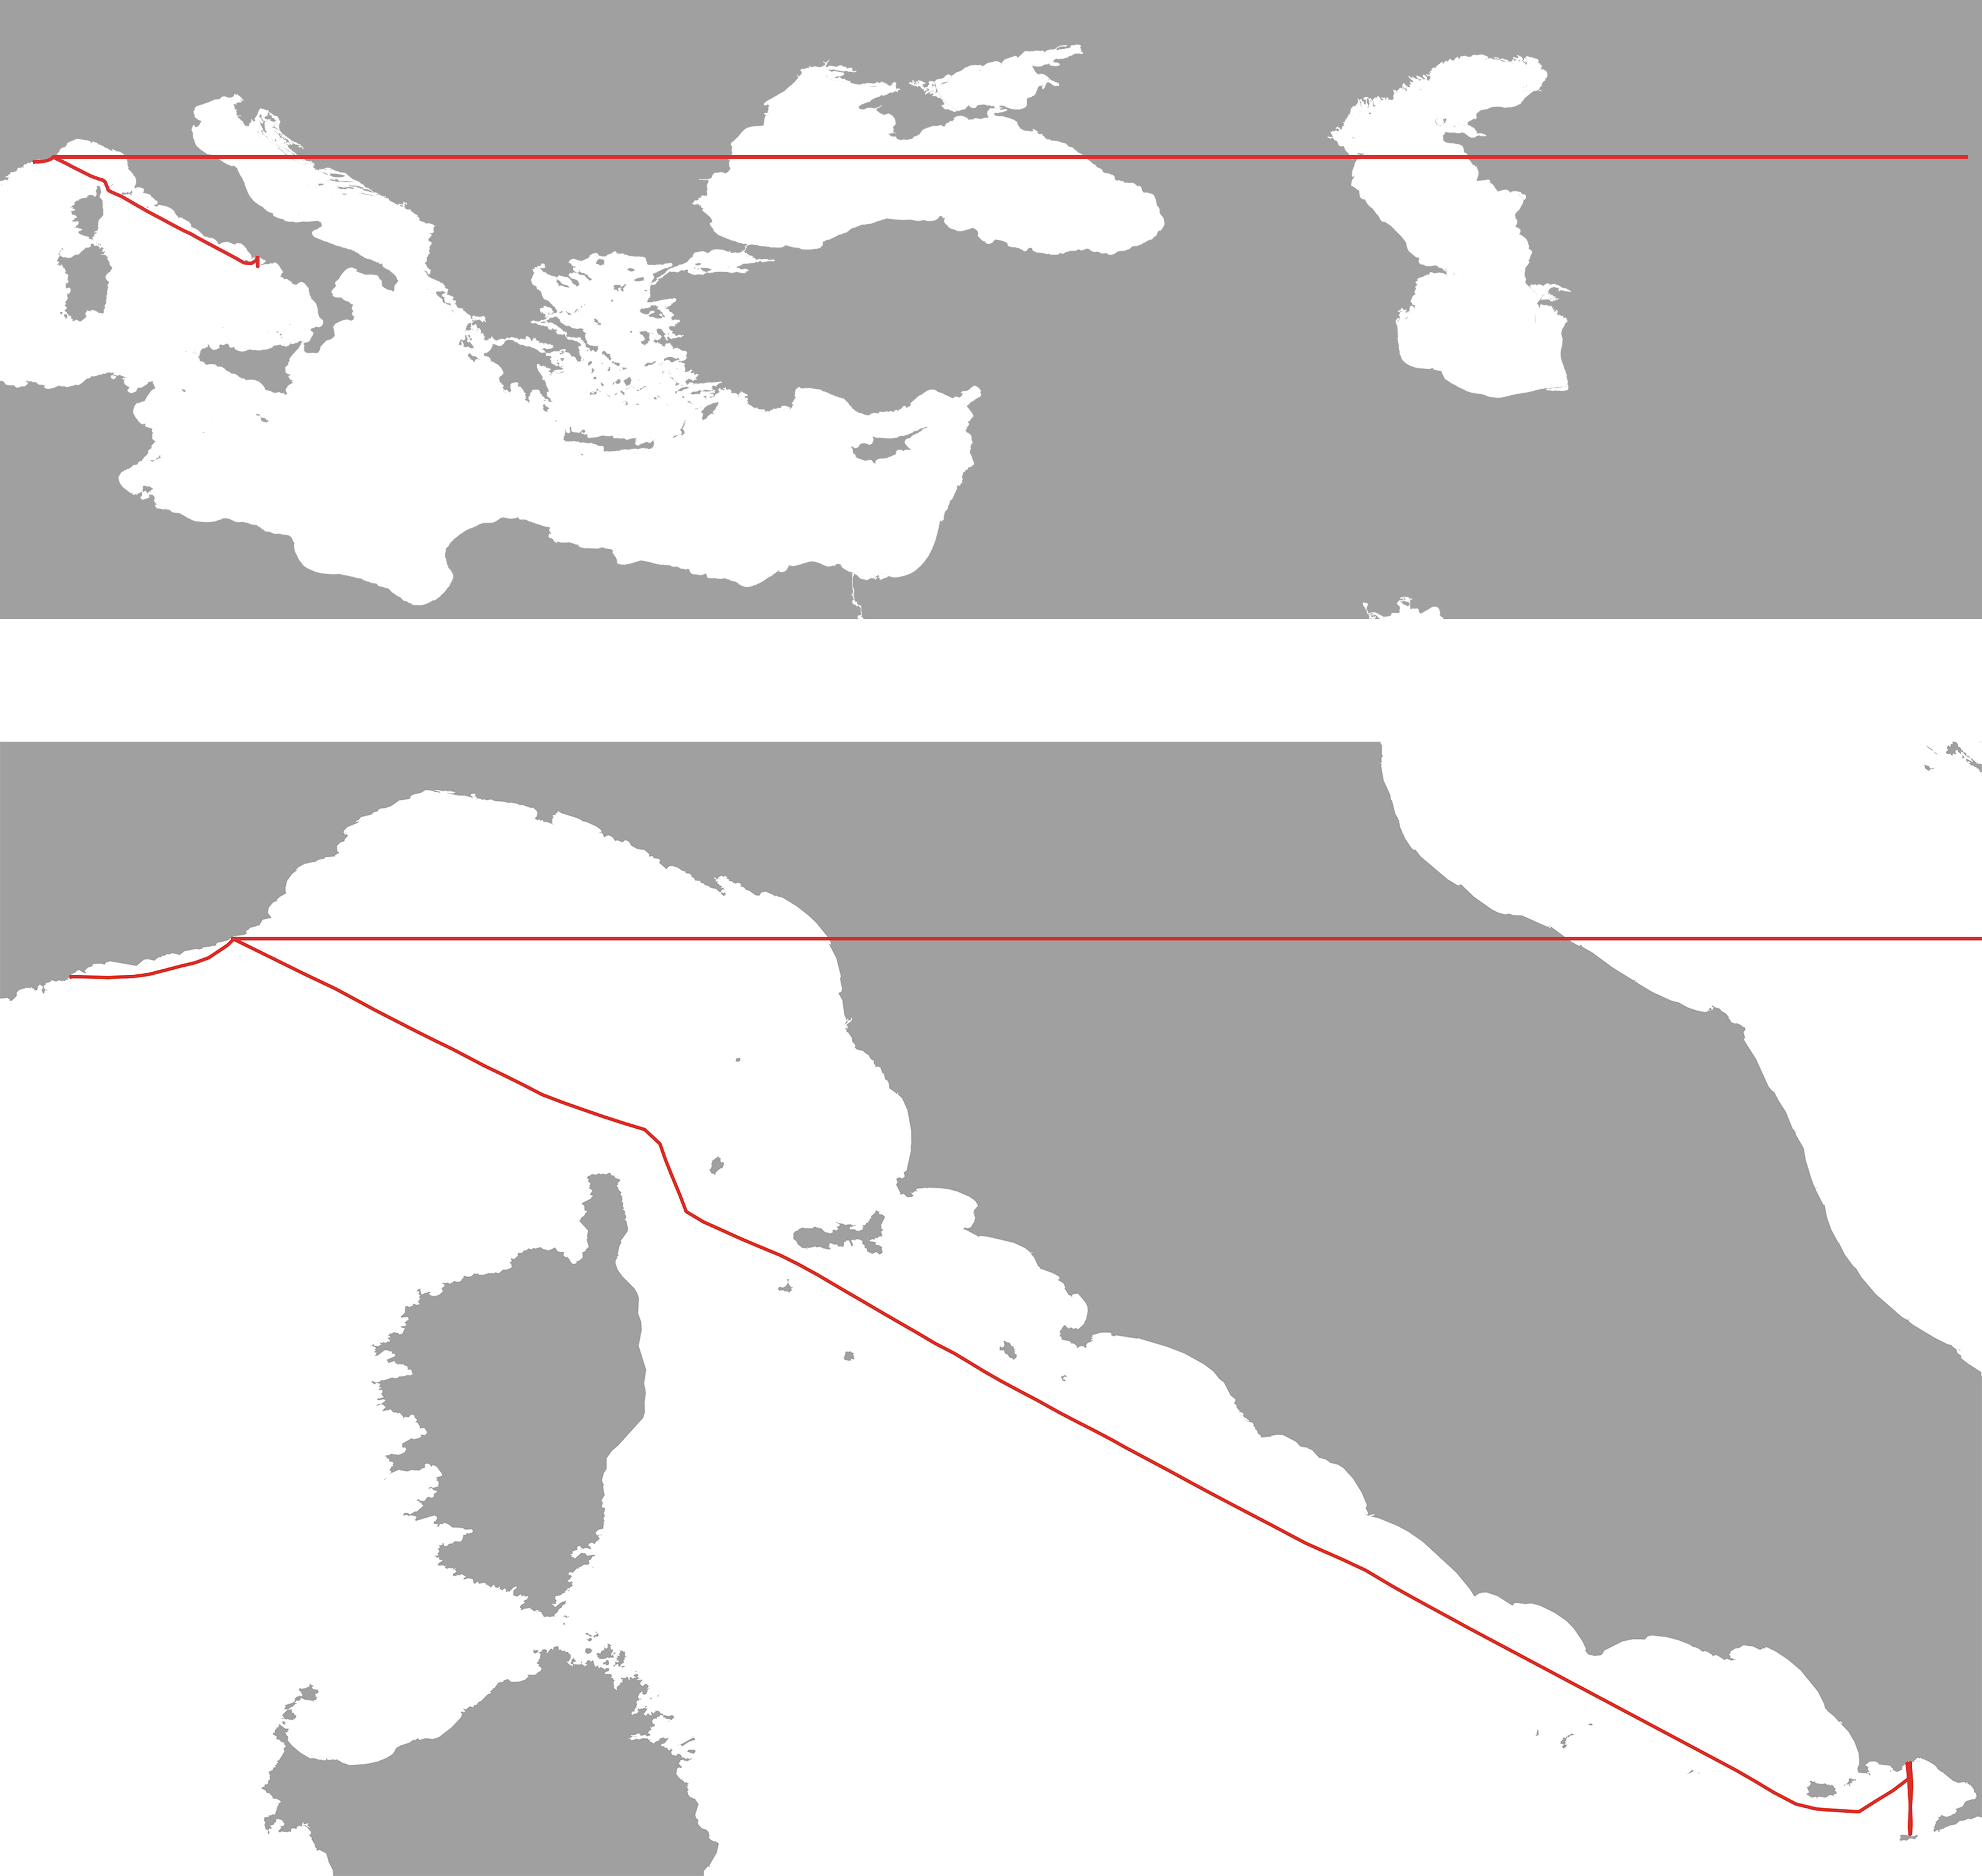
\includegraphics[width=0.7\textwidth]{figures/trajectory_noise/noisy_trajectory}
    \caption{Example showing a ``noisy'' trajectory presumably caused by GPS inaccuracy or equipment error}
    \label{fig:noisy_trajectory}
\end{figure}

An example of this issue is visualized in \cref{fig:noisy_trajectory} which shows a voyage starting in Monaco and ending in Naples, Italy. During a stopping point in northern Italy, the vessel transmitted two longitude values placing the vessel in the middle-east while then continuing the journey arriving in Naples, Italy. This issue is presumably caused by issues with the GPS signals sent by the \acrshort{ais} transmitter on board the vessel or by some other equipment error. Excluding the fluctuated segment of the trajectory, the remaining trajectory is completely valid, thus, if it is possible to remove the invalid part of the trajectory, the remainder could be further used in the analysis. Therefore, ``noise filter'' was employed to detect and cut away fluctuations in otherwise valid trajectories.

\begin{figure}[htbp]  % order of priority: h here, t top, b bottom, p page
    \centering
    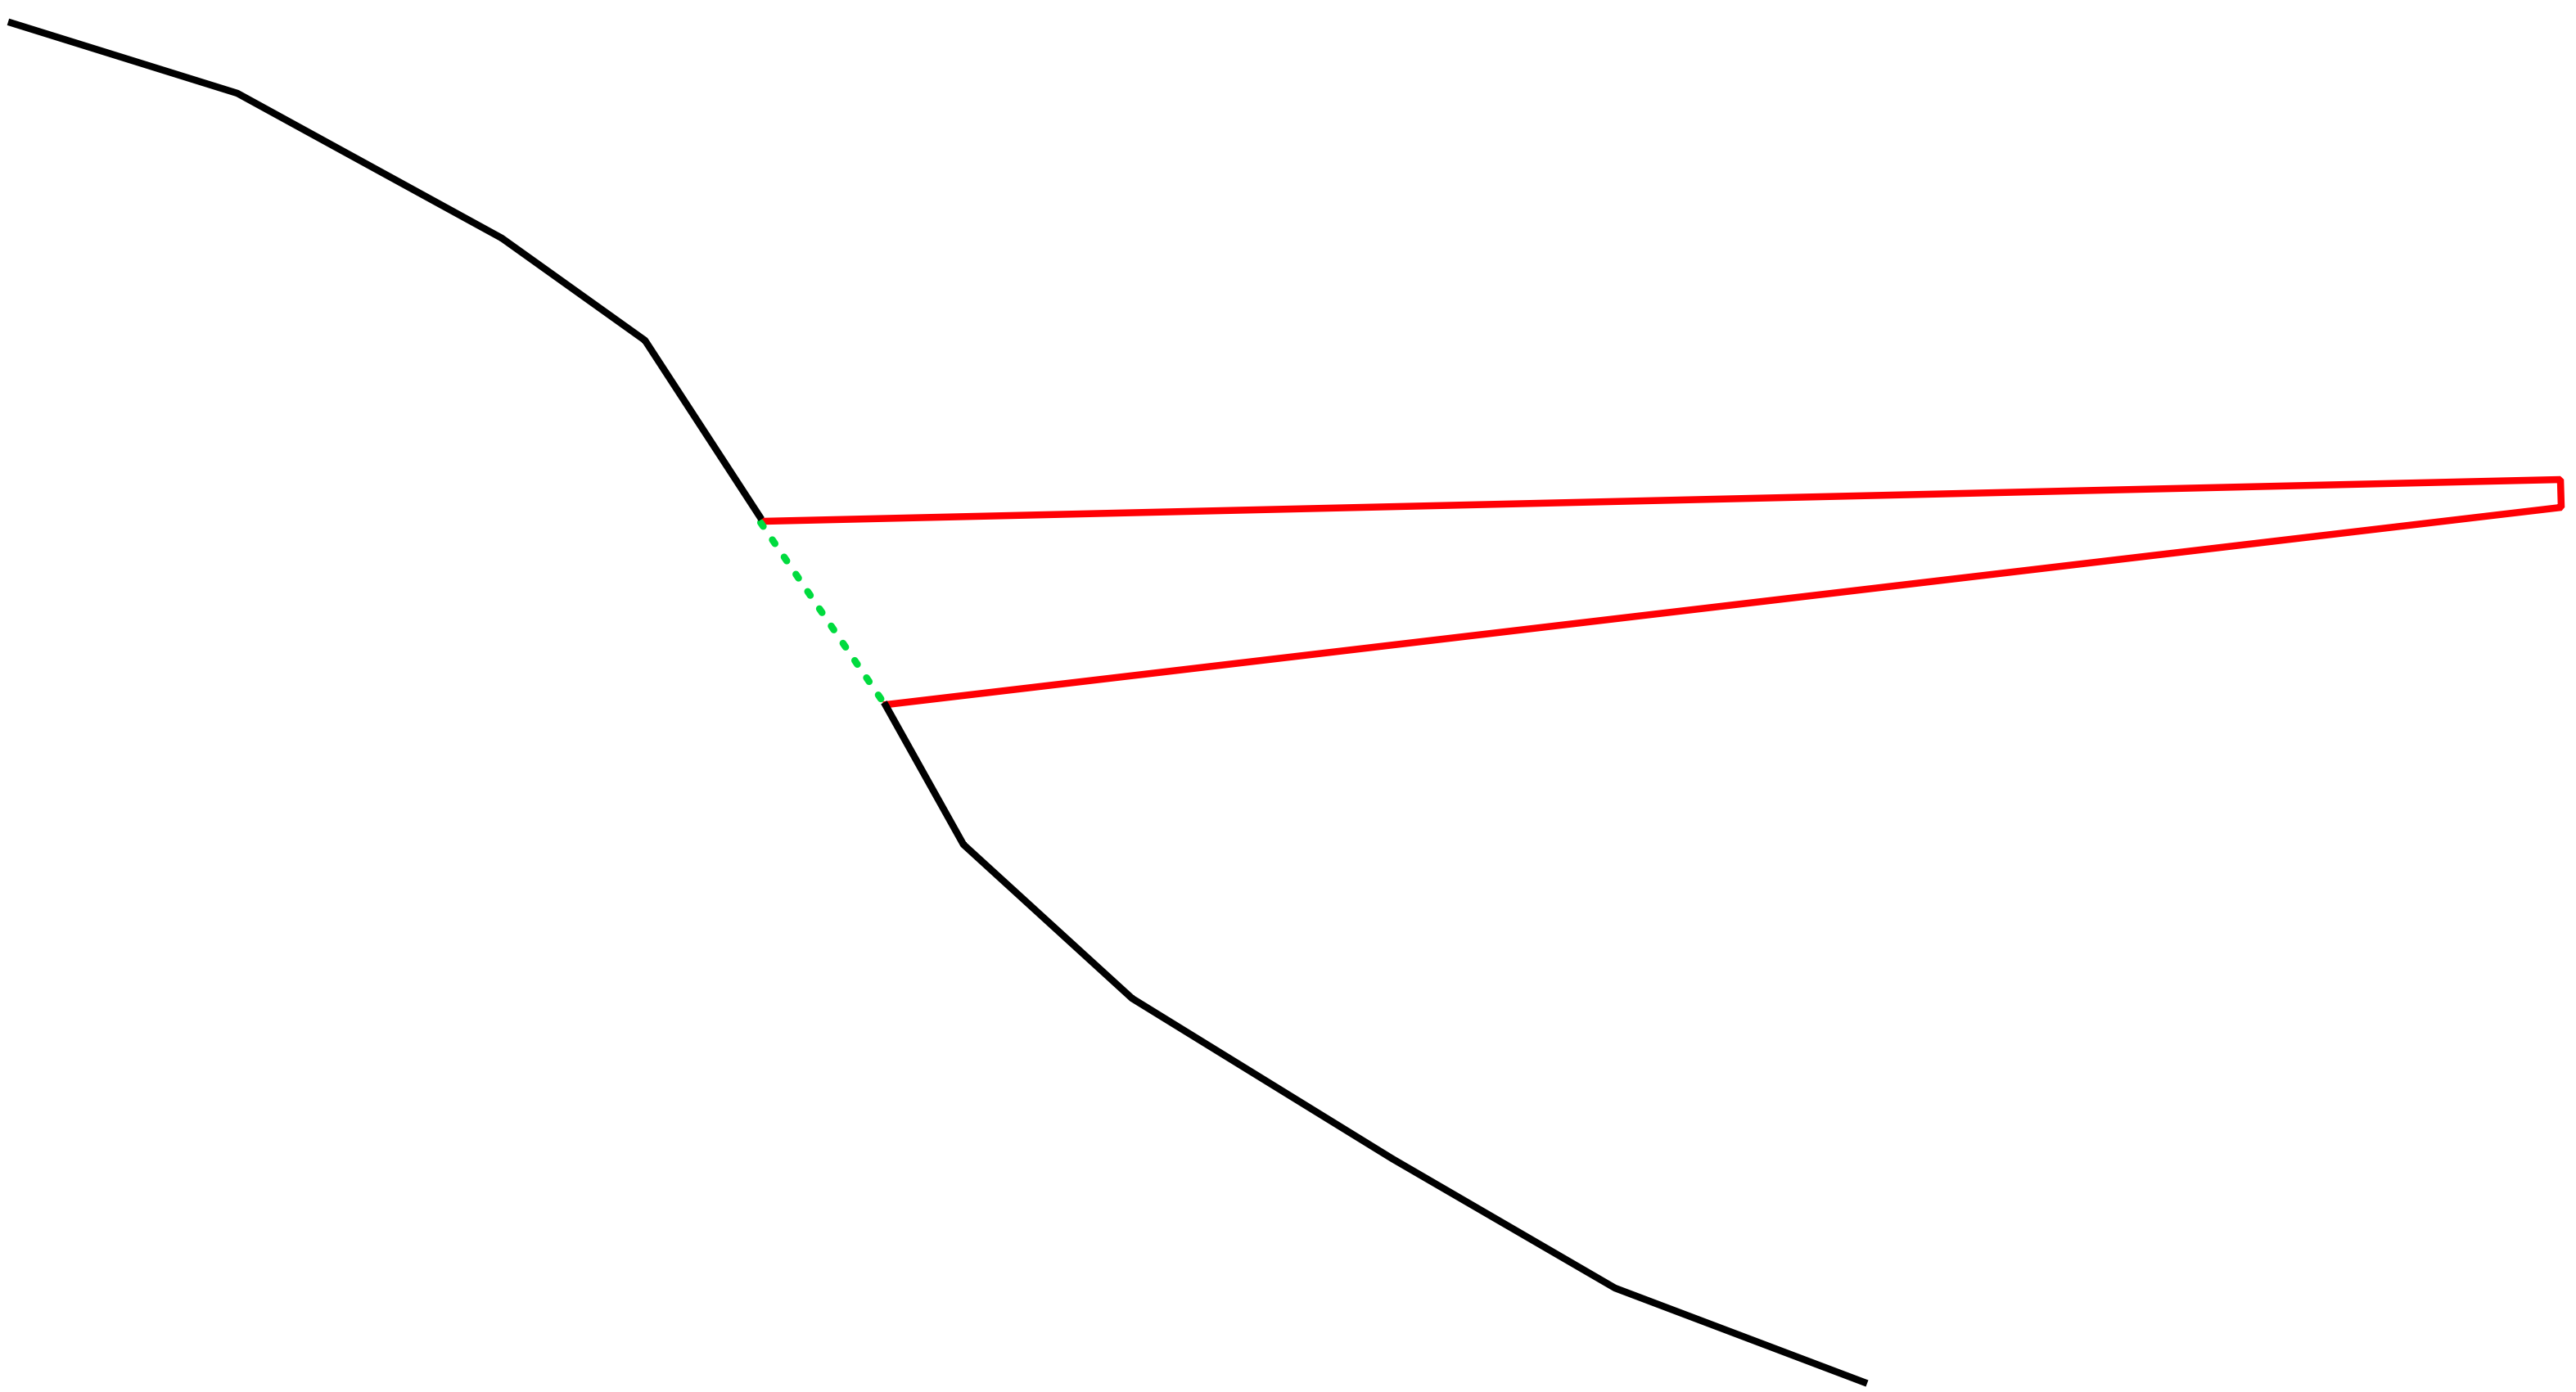
\includegraphics[width=0.6\textwidth]{figures/trajectory_noise/noise_filter}
    \caption{Noise filter algorithm cutting out points in a trajectory detected as noise. The red segment is cut out and the black segments are tied together as shown with the green dotted line.}
    \label{fig:noise_filter}
\end{figure}

\begin{figure}[htbp]  % order of priority: h here, t top, b bottom, p page
    \centering
    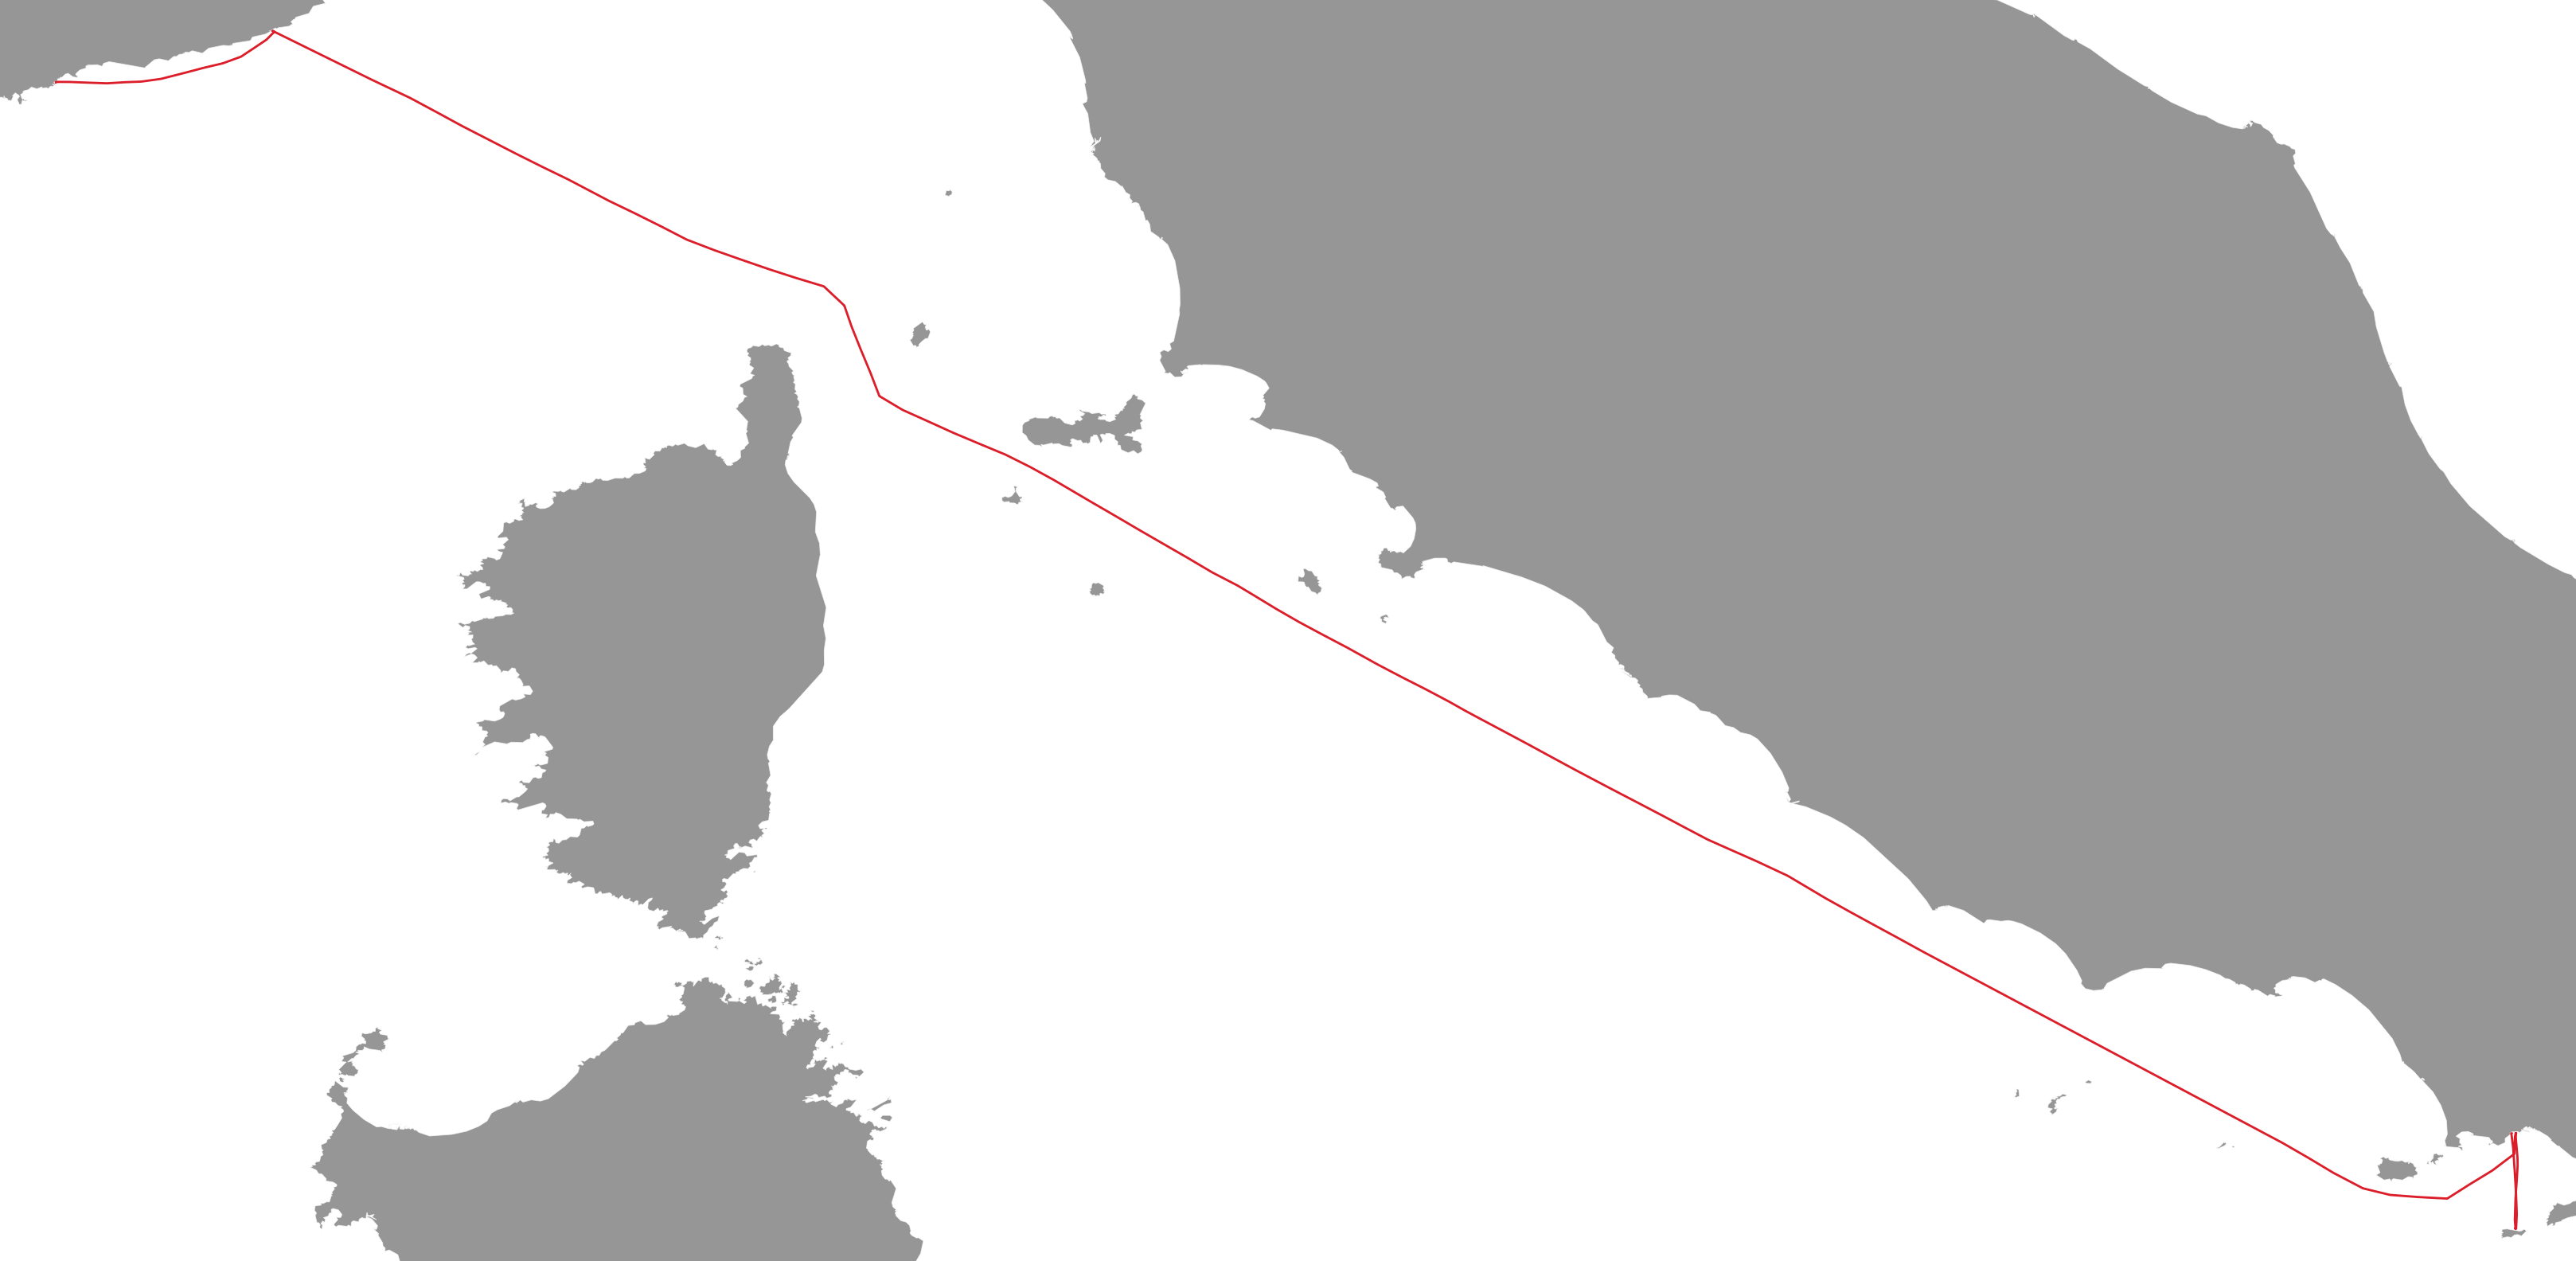
\includegraphics[width=0.8\textwidth]{figures/trajectory_noise/filtered}
    \caption{The example trajectory shown \cref{fig:noise_filter} from Monaco to Naples after noise filtering.}
    \label{fig:noise_filtered}
\end{figure}

The noise filtering employed in the trajectory builder is shown in \cref{fig:noise_filter} where the red segment fluctuates in an otherwise valid trajectory and is therefore excluded from the remaining trajectory. For every point in the trajectory, the algorithm checks the distance between the current and the next point as well as the time difference between the two points. Using the distances in space and time, it calculates the speed the vessel would require to travel from the first to the second point. If the speed required was more than 50 knots, the segment was invalid. The next point is then compared to the first to see if there is a possible valid path to the third point. If there is, the second point is disregarded from the trajectory. The algorithm is given a tolerance of four invalid points before it disregards the entire trajectory. \cref{lst:noise_filter} shows the function used to find the next valid point in a trajectory, if it returns an error, the trajectory is disregarded. \cref{fig:noise_filtered} shows the same trajectory from \cref{fig:noisy_trajectory} after the following algorithm has filtered out fluctuating segments.

\begin{lstlisting}[
    caption={Golang code used find the next valid point for any given point in a trajectory.},
    label=lst:noise_filter,
    language=Go
]
// nextValidPoint returns the index of the next valid point checking distances to
// every point within tolerance. If no valid distances were found wihin tolerance,
// it returns an error. If the last point in trajectory was reached, -1 is returned
func nextValidPoint(start, tolerance int, positions []VesselPosition) (int, error) {
	a := positions[start]
	for j := start + 1; j <= start+tolerance; j++ {
		if j >= len(positions) {
			return -1, nil
		}

		n := positions[j]
		dist := DistanceHaversine(Point{a.Lon, a.Lat}, Point{n.Lon, n.Lat})
		// use the absolute value in case the trajecotory is not sorted
		timeDiff := math.Abs(float64(n.Timestamp - a.Timestamp))

		// calculate the required speed to reach the given point with the
		// given time difference * 1.94385 to konvert m/s to knots
		requiredSpeed := (dist / timeDiff) * 1.94385
		// if required speed was >= 50kt, move on to next point
		if requiredSpeed < 50.0 {
			return j, nil
		}
	}
	// no reasonable distances were found within tolerance
	return -1, errors.New("trajectory segment too noisy")
}
\end{lstlisting}

Finally, when the voyage trajectories have been constructed and validated, they are collected in a database table called transition voyages which contains the following relevant attributes:

\begin{itemize}
    \item imo - identifier for the vessel.
    \item mmsi - identifier for the vessel.
    \item departure port - voyage departure port's locode.
    \item departure timestamp - the time of departure.
    \item arrival port - voyage arrival port's locode.
    \item arrival timestamp - the time of arrival.
    \item trajectory - 3D linestring with longitude, latitude, and timestamp for each point.
\end{itemize}

It is worth noting that the trajectories are stored as 3D PostGIS linestring geometries where each point contains a \textit{x}, \textit{y}, and \textit{z} value where the \textit{z} value holds the UNIX timestamp of the positional record. Keeping the timestamp value is necessary for sampling trajectories based on time, and keeping the time values stored directly in the trajectory geometry saves an extra table for trajectory points.

\section{Data processing for \acrfull{ml}}

After the initial data set has been collected and vessel voyages have been defined and constructed, the next step is to build the final training dataset to be used for analysis and \acrfull{ml}. This section describes every step in the process used to construct this dataset based on data described up to this point in this chapter.

\subsection{Trajectory sampling}

Vessels transmit \acrshort{ais} records at different frequencies and messages collected via satellite are collected at different frequencies as the satellites have different orbits. Therefore the frequency, or density, or records in trajectories can not be expected to be standardized. Furthermore, as vessels travel at different speeds, two trajectories with similar start and end positions might have different shapes and contain a different number of points. In addition, as discussed in \cref{sec:vessel_voyage_definition}, one disadvantage of relying on \acrshort{ais} navigational statuses is that vessels can stop during a voyage for different reasons before arriving at their final destinations. Whenever a vessels stops moving or moves slowly, many \acrshort{ais} records are transmitted in clusters which cause noise and redundant data in the constructed trajectories.

\begin{figure}[htbp]  % order of priority: h here, t top, b bottom, p page
    \centering
    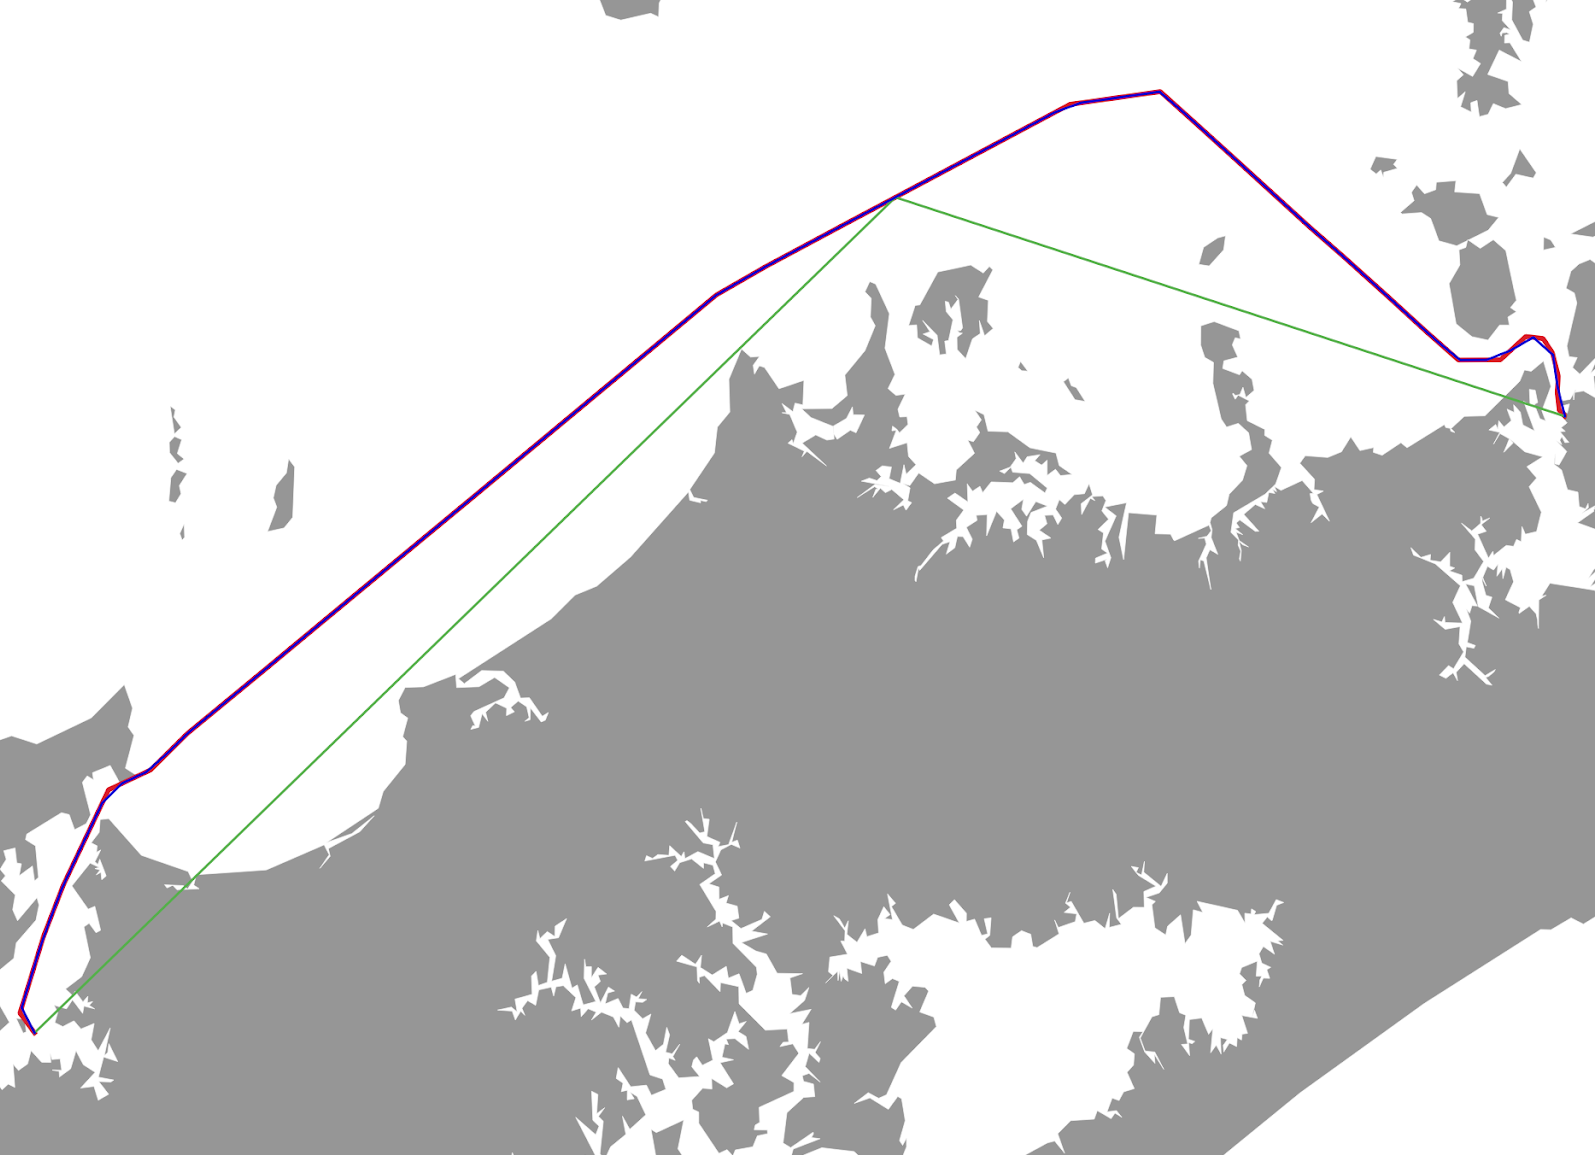
\includegraphics[width=0.8\textwidth]{figures/trajectory_sampling}
    \caption{Example of a trajectory sampled by both distance (2 km) and time (6 hours). The red trajectory is not sampled, the blue is sampled based on 2 km in distance, and the green is sampled based on six hour time intervals.}
    \label{fig:trajectory_sampling}
\end{figure}

The proposed solution includes using similarity between trajectories to predict traveling vessels' destination ports, therefore, in order to make the trajectories more comparable a sampling step was added in the process of constructing the training data. There were two main approaches considered for trajectory re-sampling, namely sampling based on distance and time. When sampling based on a predefined distance, each subsequent point in a trajectory must be the same distance apart from each other. When sampling based on time, one position is extracted from a trajectory for every given unit of time. For instance, if sampling based on time with a six hour sample rate, starting from the first point, every position within six hour intervals are grouped and all positions within each group are dropped except for the first one. Both methods achieve the goal of making trajectories more comparable, however, sampling based on time simplifies, or reduces, the amount of data in each trajectory the most. It also provides an indication of trajectory duration implicitly through the trajectory length, or the number of points in a trajectory.

For these reasons, throughout the rest of the implementation, sampling is done based on time using a time interval of six hours. It is worth noting that for trajectories shorter than six hours, only the first and last point in the trajectory is returned reducing the trajectory to a straight line. In order to sample any trajectory based on either time or distance, a Golang package was written called ``sampler'' which can parse and handle both 3D trajectories including timestamps for time sampling, and 2D trajectories for distance sampling. The complete code for this package can be found in \cref{app:sampler}. \cref{lst:trajectory_sampler} shows an extract from this package of the function used to resample trajectories based on time.

\begin{lstlisting}[
    caption={Golang code from a sampler package written to sample a trajectory based on time.},
    label=lst:trajectory_sampler,
    language=Go
]
// resampleTime resamples trajectory based on s.SampleRate given in hours.
// Extracts the first position within intervals based on sample rate
func (s *Instance) resampleTime() (string, error) {
	var err error
	trajectory, err := s.parse3DTrajectory()
	if err != nil {
		return "", err
	}

	intervals := s.getTimeIntervals(trajectory)
	reducedCoords := []geom.Coord{}
	coords := trajectory.Coords()

	// within each interval add the first coord to reducedCoords
	for _, interval := range intervals {
		var first *geom.Coord

                // get first coord in interval
		for i := range coords {
		        // roundTime uses s.SampleRate when rounding
			coordInterval := s.roundTime(int64(coords[i][2]))
			if coordInterval == interval {
				first = &coords[i]
				break
			}
		}
		if first != nil {
			reducedCoords = append(reducedCoords, *first)
		}
	}

	// if the last coord wasn't the last in reduced, add it
        lastReduced := reducedCoords[len(reducedCoords)-1]
	if !lastReduced.Equal(geom.XYZ, coords[len(coords)-1]) {
		reducedCoords = append(reducedCoords, coords[len(coords)-1])
	}
	if len(reducedCoords) <= 1 {
		return "", errors.New("too few points in sampled trajectory")
	}
	reduced, err := geom.NewLineString(geom.XYZ).SetCoords(reducedCoords)
	if err != nil {
		return "", err
	}

	return geomwkt.Marshal(reduced)
}
\end{lstlisting}

The function listed in \cref{lst:trajectory_sampler} is used in a batch process that samples every voyage's trajectory and keeps the sampled voyages in a separate table called ``sampled transition voyages''. The batch process extracts 5000 voyages at a time, samples their trajectories, and batch-inserts them into the separate table. By not mutating the original voyage data, different sampling methods can be applied and tested to find differences in trajectory comparisons.

\subsection{\acrfull{mstd}}

In order for the proposed solution to take into account both geographical trajetories as well as additional vessel information for predictions, in the training set, the trajectories have been abstracted into the categorical and numeric values \acrfull{mstd}, the similarity value for the \acrshort{mstd}, and then the length of the trajectory. The \acrshort{mstd} for a given voyage is found by measuring the similarity between the given voyage's trajectory and every historical trajectory in the sampled transition voyages table. The most similar trajectory is found using a given trajectory similarity measurement, and its destination and similarity value is added to the final dataset. As described in \cref{sec:trajectory_similarity}, there are several different trajectory similarity measurements available, however, for this thesis the \acrfull{sspd} is used to calculate the \acrshort{mstd} values. However, the process and the dataset is structured in such a way that it is possible to use different similarity measurement methods in this process. For instance, the \acrshort{ml}-based method proposed in \cite{Zhang2020AISApproach} achieved good performance for similarity based predictions, thus it could be replicated and used to calculate the \acrshort{mstd} values for this approach.

\begin{figure}[htbp]  % order of priority: h here, t top, b bottom, p page
    \centering
    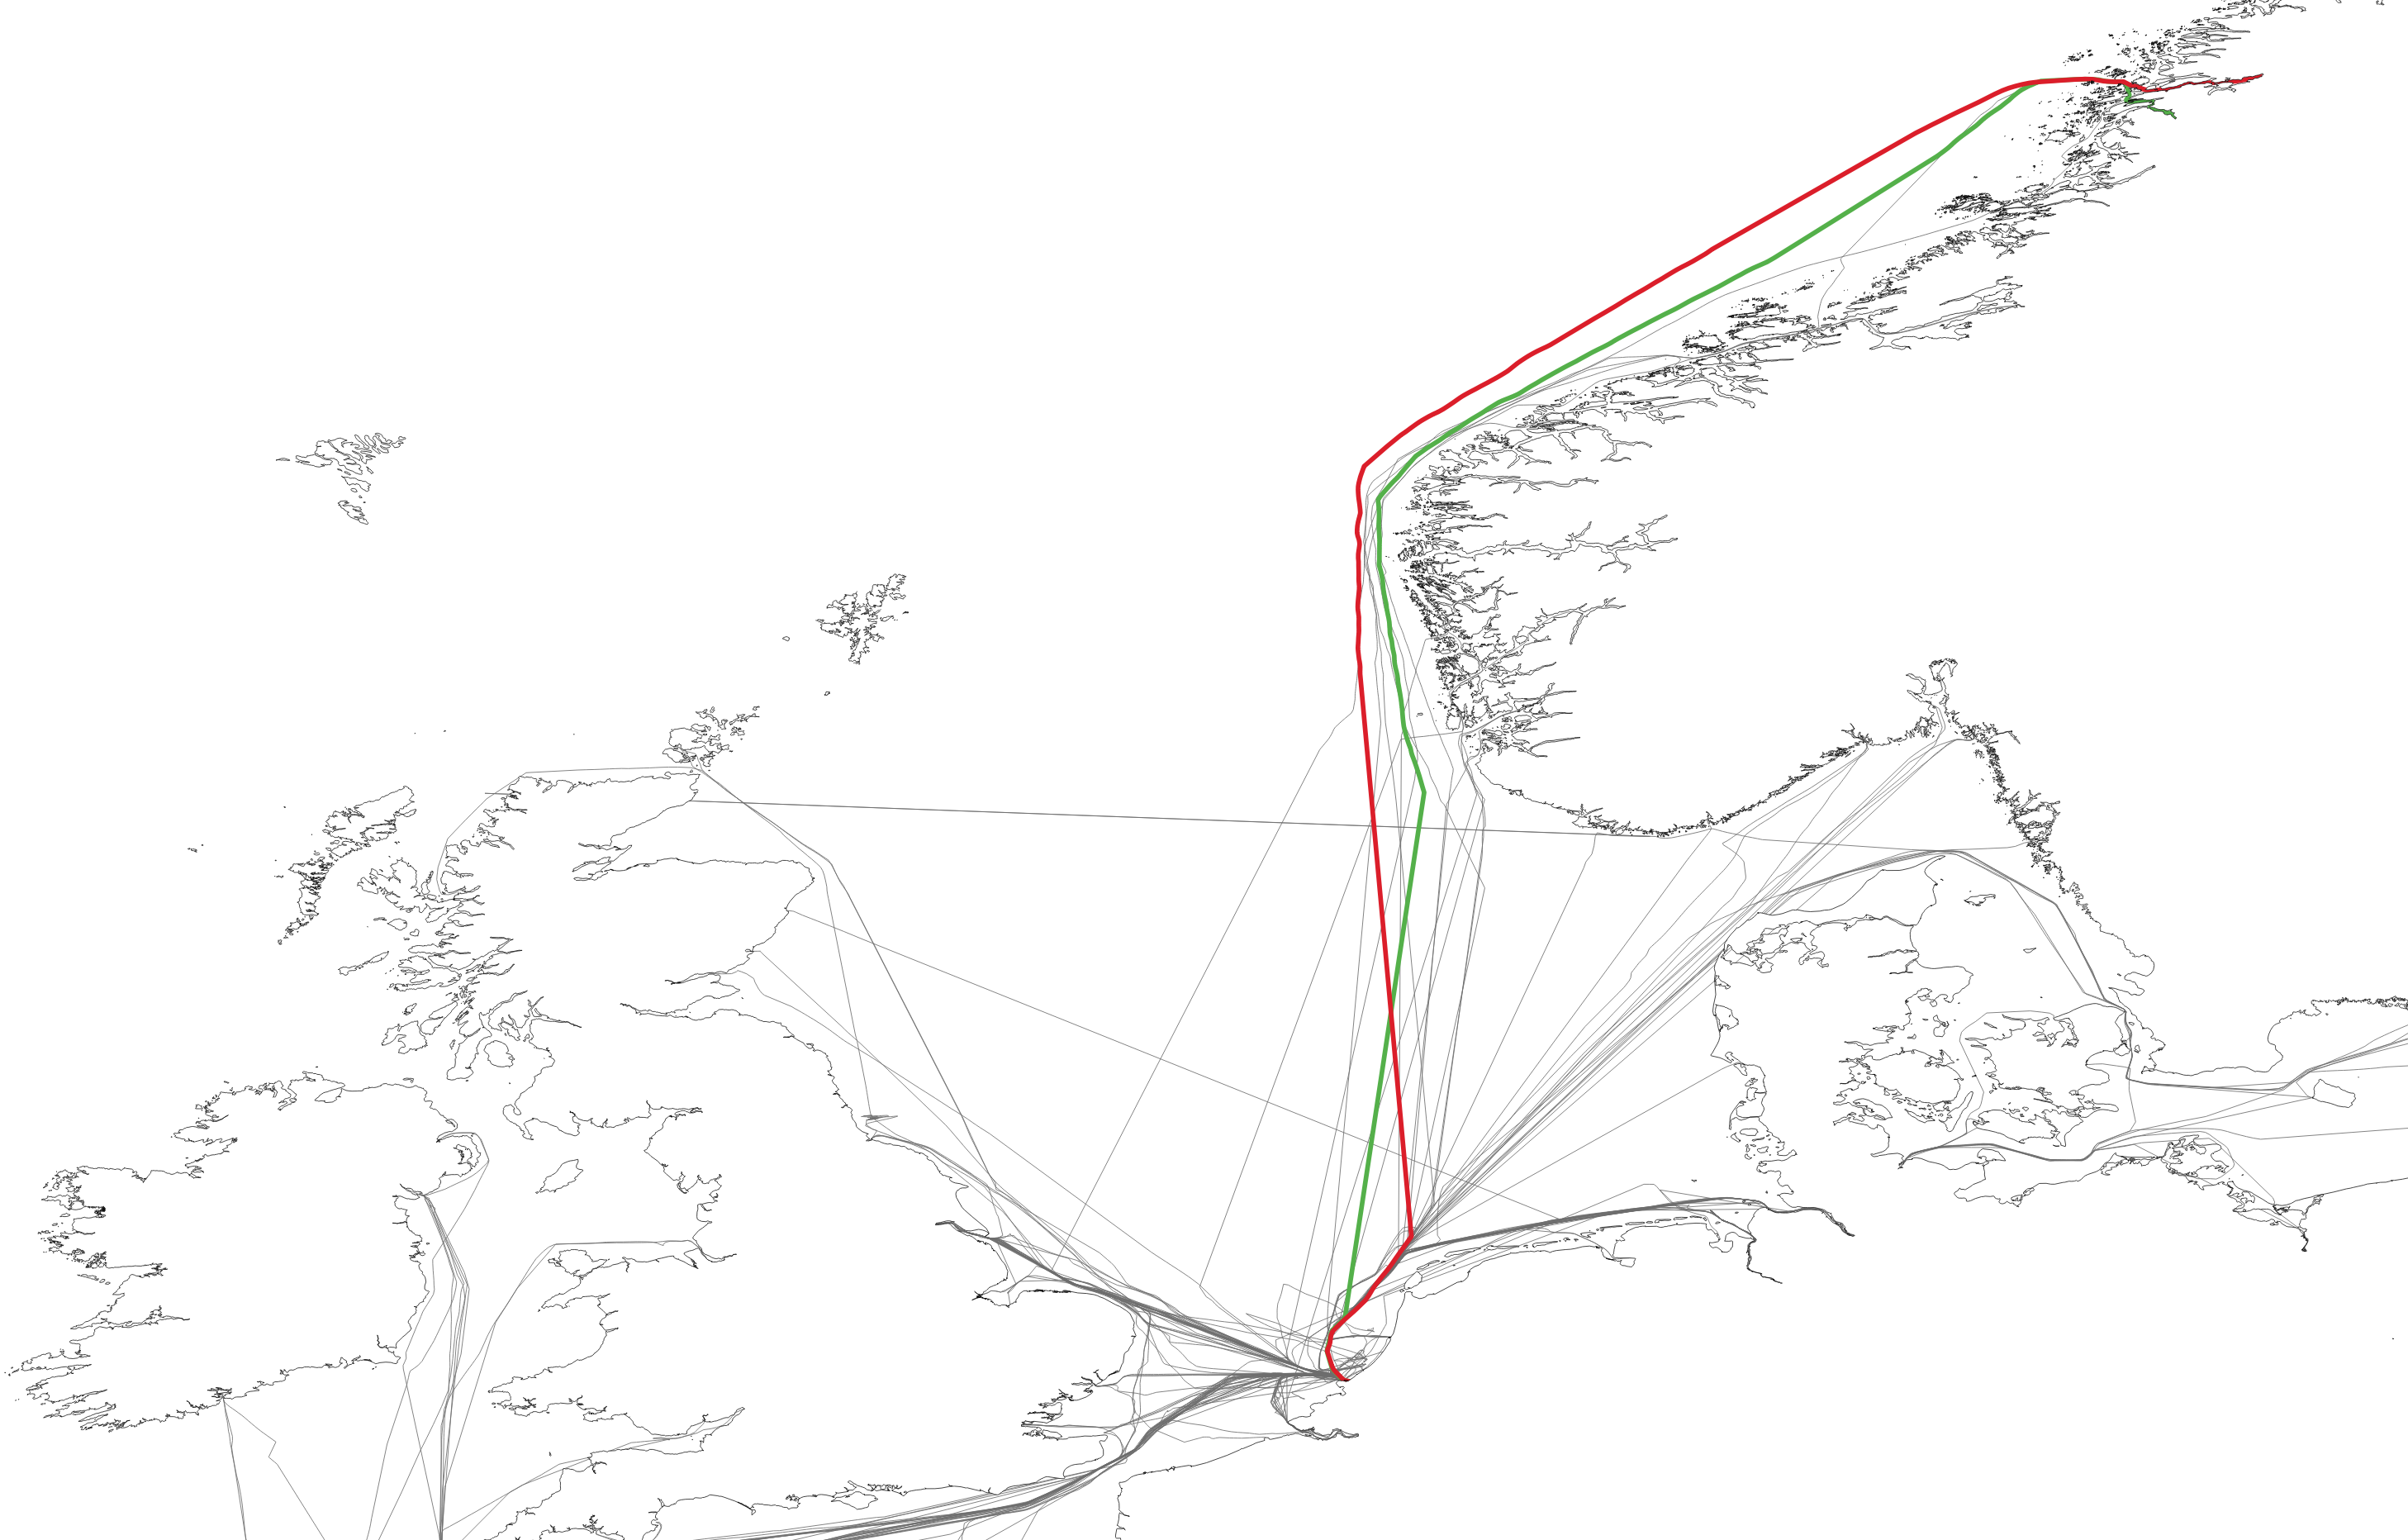
\includegraphics[width=1.0\textwidth]{figures/mstd}
    \caption{Example of \acrshort{mstd} for a given historical trajectory where the red line is the given trajectory and the green line is the most similar historical trajectory.}
    \label{fig:mstd}
\end{figure}

The \acrshort{mstd} value for a given voyage is calculated in the following steps:

\begin{enumerate}
    \item Given a sampled voyage, fetch every historical voyage with the same departure port from vessels of the same segment and sub-segment.
    \item Use a given similarity measurement method, \acrshort{sspd} in this case, to calculate the similarity between the given voyage's trajectory and every historical voyage's trajectory. The given similarity measurement method must return a similarity value. For \acrshort{sspd}, this value is a Haversine distance value.
    \item Find the most similar historical trajectory, or the trajectory with the smallest similarity value.
    \item Extract the most similar historical trajectory's destination port as the \acrshort{mstd} value and extract the similarity value for future use.
\end{enumerate}

\cref{fig:mstd} shows an example of finding the most similar historical trajectory (green line) for a given voyage (red line). The given voyage departed the port of Rotterdam, and arrived in Mo i Rana, Norway. Every other historical voyage that departured Rotterdam from vessels of the same segment and sub-segment was then extracted and \acrshort{sspd} was used to find the most similar historical trajectory.

\subsection{Building ML data training set}

\begin{itemize}
    \item Batch calculating MSTD with incomplete voyages
    \item Different trajectory similarity approaches
    \item Adding more data attributes per voyage such as seasons, ballast/laden, etc\ldots
    \item Final result/structure
\end{itemize}

\subsection{Dataset imbalance}

\begin{itemize}
    \item Minority oversampling
    \item Majority undersampling
\end{itemize}

\subsection{Categorical label encoding}

\begin{itemize}
    \item Categorical values/labels must be encoded
    \item Label encoding vs one-hot encoding
\end{itemize}

\section{The final dataset summary}

The final process of creating the dataset used in the analysis can be summarized in the following steps:

\begin{itemize}
    \item Voyages are defined using time intervals provided by the vessels' \acrshort{ais} navigational status. They are constructed and stored in a voyage database table containing the full geographical trajectory, arrival and departure ports, and additional information for the traveling vessel.
    \item The voyage table's geographical trajectories are sampled, or simplified, based on a certain time interval to make trajectory comparisons easier.
    \item Every sampled historical trajectory is split into multiple parts to emulate incomplete voyages not yet arrived at a port. Furthermore, the \acrshort{mstd} is calculated for every one of these voyages. Trajectory similarity is defined using the \acrshort{sspd} algorithm, however, this data is interchangeable with other similarity measurements.
    \item Finally, the \acrshort{mstd}, similarity value, trajectory length, departure and arrival ports, and vessel segmentation information is collected and stored as the \acrshort{ml} training data.
\end{itemize}

An overview of the process described in this chapter thus far is shown in \cref{fig:dataset_overview} from the data provided by \acrfull{mo} to the final \acrshort{ml} training data.

\begin{figure}[htbp]  % order of priority: h here, t top, b bottom, p page
    \centering
    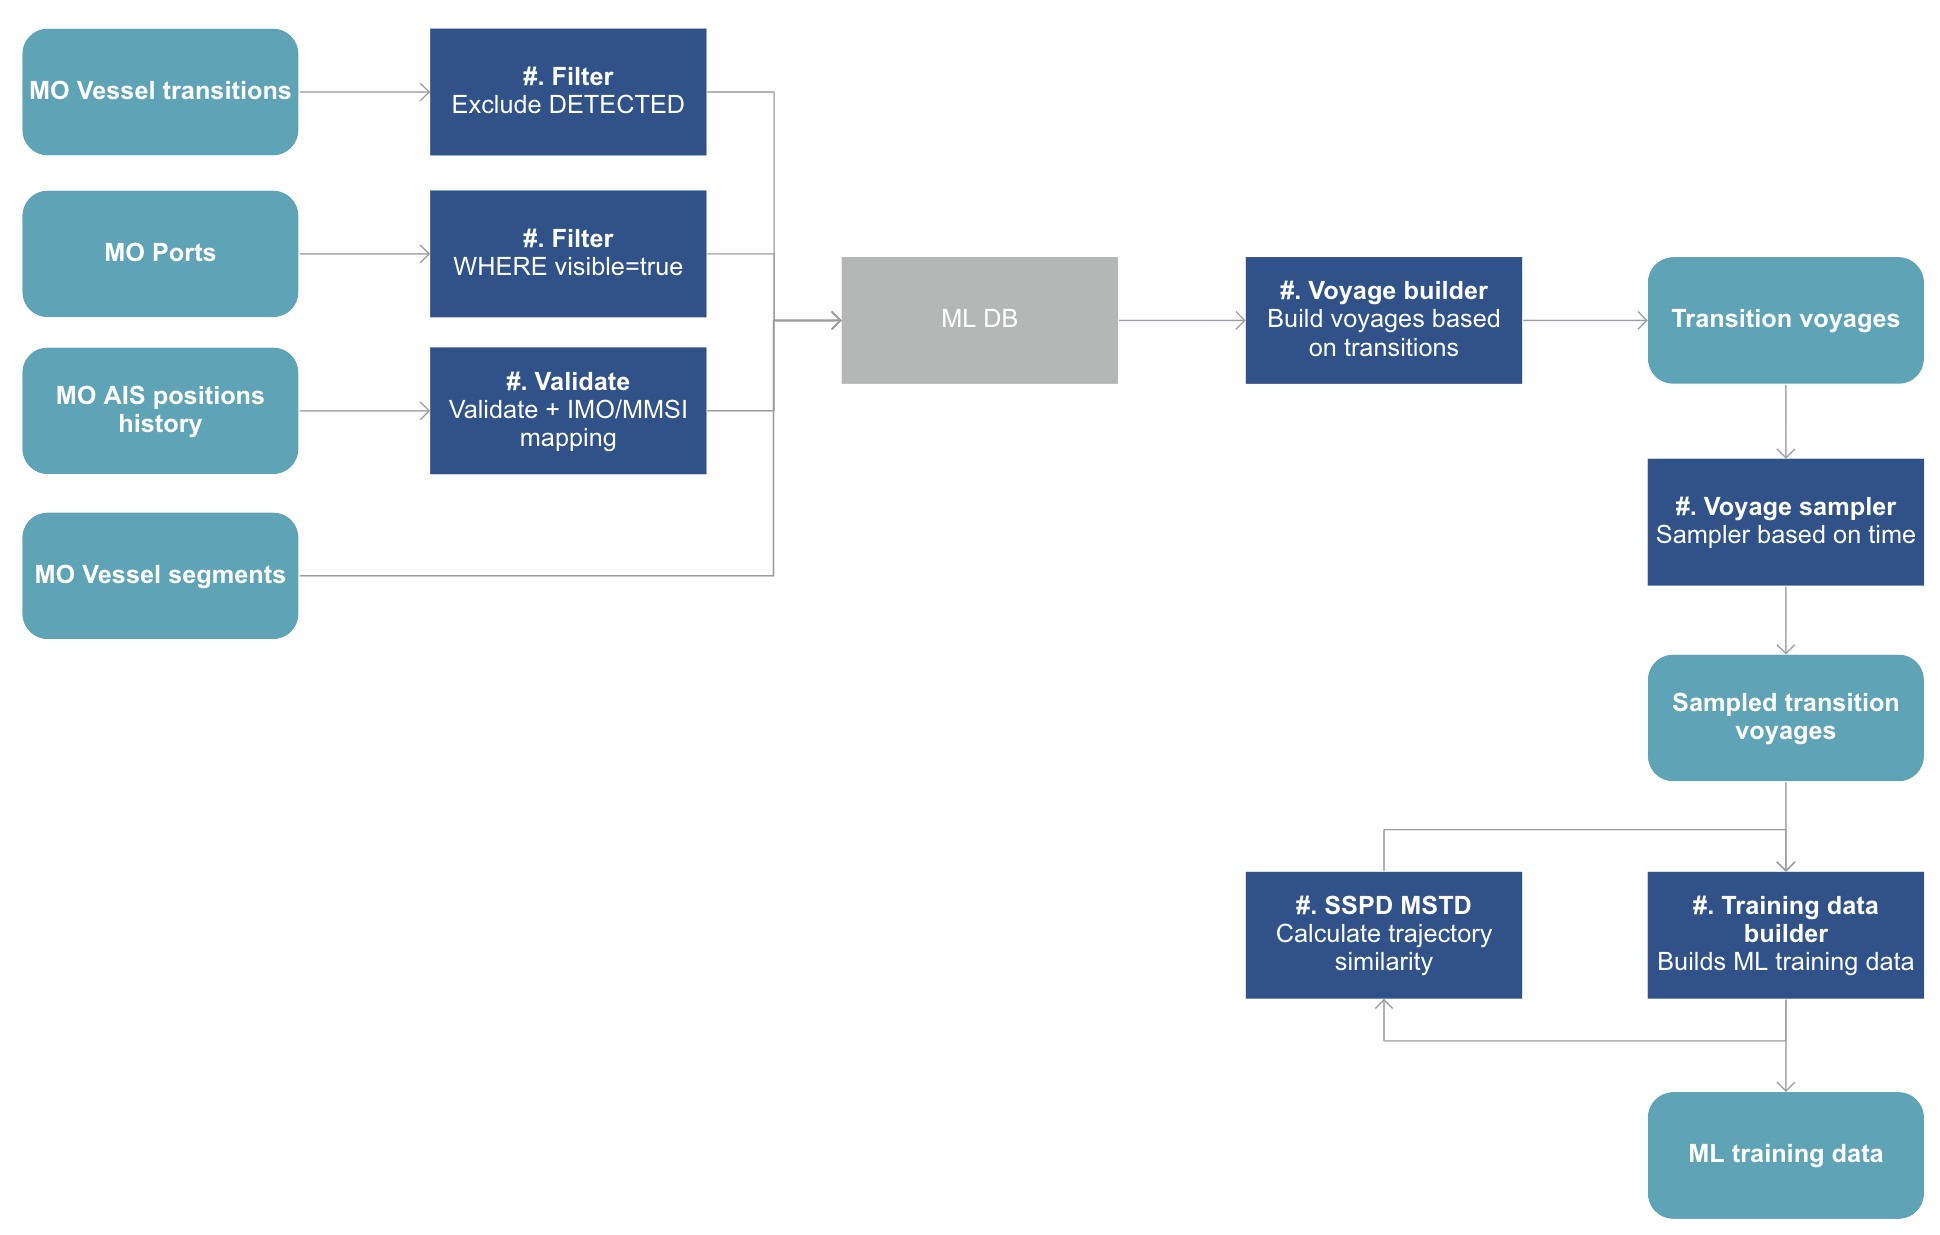
\includegraphics[width=1.0\textwidth]{figures/dataset_overview}
    \caption{Overview of the process used to construct the dataset used in further analysis and \acrshort{ml}.}
    \label{fig:dataset_overview}
\end{figure}

The final dataset is collected in a database table called \acrshort{ml} training data, and it contains the following attributes:

\begin{table}[htbp]
    \centering
    \begin{tabularx}{1.0\textwidth}{p{1.0in} p{0.75in} X}
        \bfseries{Column} & \bfseries{Type} & \bfseries{Description} \\ \toprule
        id & serial int & unique identifier \\ \midrule
        voyage\_id & int & the original voyage id from sampled transition voyages \\ \midrule
        imo & int & identifier for the traveling vessel\\ \midrule
        mmsi & int & identifier for the traveling vessel\\ \midrule
        segment & string & the vessel's segment \\ \midrule
        sub\_segment & string & the vessel's sub-segment \\ \midrule
        departure\_port & string & \gls{locode} of the vessel's departure port \\ \midrule
        trajectory\_length & int & number of points in the sampled trajectory \\ \midrule
        sspd\_mstd & string & \gls{locode} of the \acrshort{mstd} value for the voyage trajectory \\ \midrule
        sspd\_dist & int & similarity value between the voyage trajectory and the most similar historical trajectory   \\ \midrule
        arrival\_port & string & \gls{locode} of the vessel's arrival port \\ \bottomrule
    \end{tabularx}
\caption{Final structure of the ml\_training\_data database table.}\label{tab:ml_training_data}
\end{table}


\section{ML-based training and destination prediction}

\subsection{Model selection}

\begin{itemize}
    \item Tree-based classifiers
    \item Multi-layered perceptrons classifiers
    \item Support-vector machines
    \item Multi-class classifiers vs OneVsRest binary classifiers
\end{itemize}

\subsection{Configuration and parameter optimization}

\subsection{Training}

\subsection{Evaluation process and metrics}

\begin{itemize}
    \item X-Folder-cross-validation
    \item Metrics: F1, precision, recall, AUC, vs accuracy
    \item Computing performance?
    \item How fast is it to compute the next destination of every vessel in the world
\end{itemize}

\section{Vessel destination prediction method summary}

Given the final trained model, the overall prediction process for a single traveling vessel can be conceptualized using the following steps:

\begin{itemize}
    \item The current trajectory of the traveling vessel is collected using \acrshort{ais} records ranging from the last transmitted \textit{``MOORED''} status to its current position along with the id (\gls{locode}) of the departure port where it was moored and the vessel's segmentation values.
    \item The vessel's trajectory is then sampled based on a predefined time interval, then compared to every historical outgoing trajectory from the same departure port from vessels of the same segment and sub-segment to establish the \acrfull{mstd}.
    \item The vessel's segment, sub-segment, departure port, trajectory length, \acrshort{mstd}, and the \acrshort{mstd} similarity value is then passed to a \acrshort{xgb} model that predicts the traveling vessel's arrival port.
\end{itemize}
